\documentclass{beamer}
\usetheme{Warsaw}
\usepackage{tabularx}

\usepackage{graphicx}

\title{FLUSH+RELOAD vs. Privacy}

\author{Taylor Hornby \and John Aycock\footnote{He hasn't seen these
slides yet, so if my presentation sucks it's not his fault.}}

\begin{document}
% =============================================================================
% TITLE PAGE
% =============================================================================
    \frame{\titlepage}

% =============================================================================
% SIDE CHANNELS
% =============================================================================
\begin{frame}
    \frametitle{Side Channel Attacks}
    Your code might do the right thing, but it still leaks the key.
    \begin{itemize}
        \item Radio.
        \item Power.
        \item Sound.
        \item Time.
        \item \textbf{FLUSH+RELOAD from Yuval Yarom and Katrina Falkner}
    \end{itemize}
\end{frame}

% =============================================================================
% FLUSH+RELOAD
% =============================================================================

\begin{frame}
    \frametitle{\textsc{Flush+Reload}}
    \framesubtitle{Cache Architecture}

    \begin{itemize}
        \item Memory is divided into \textbf{cache lines} (64 bytes).
        \item Caching is based on the \textbf{physical address}.
        \item A cache line is either cached or not cached.
        \item L3 cache is shared between cores.
    \end{itemize}

    \begin{center}
        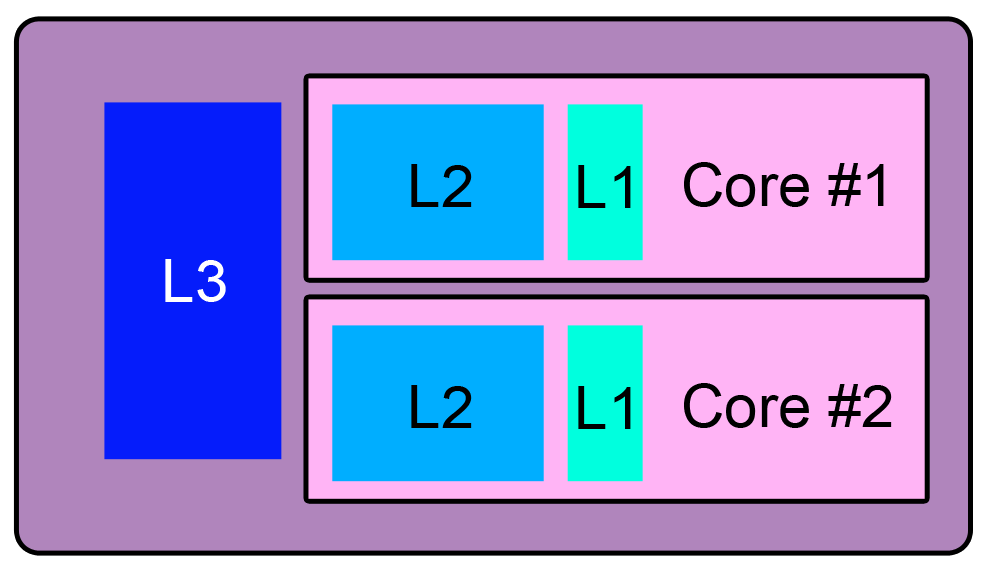
\includegraphics{cachearch.png}
    \end{center}

\end{frame}

\begin{frame}
    \frametitle{\textsc{Flush+Reload}}
    \framesubtitle{Sharing Physical Memory}

    \begin{center}
        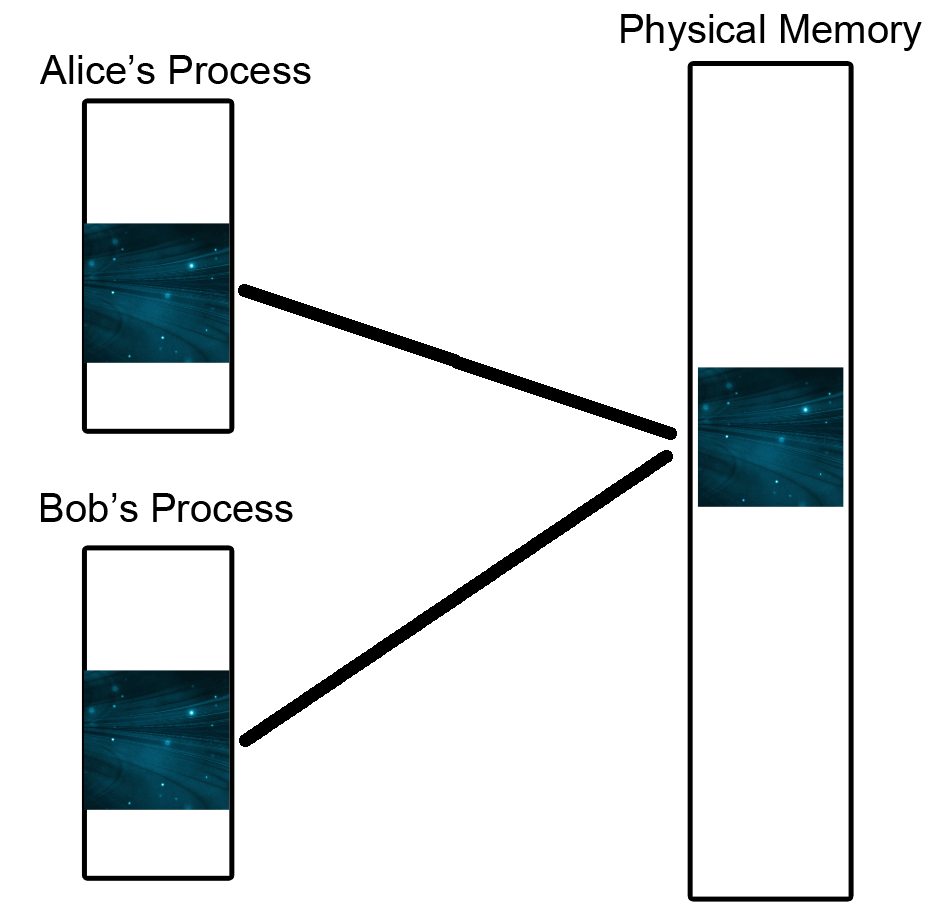
\includegraphics{codesharing.png}
    \end{center}

    \begin{itemize}
        \item Physical memory is \textbf{shared for program code}.
        \item ``Cachedness'' of Alice's and Bob's code is the same.
        \item When Alice runs code, it gets loaded into the cache.
        \item Bob can tell what code Alice is running.
    \end{itemize}
\end{frame}

\begin{frame}
    \frametitle{\textsc{Flush+Reload}}
    \framesubtitle{Spying on A Program}

    \textbf{Input:} Some \textbf{probes} (cache line addresses) Bob wants to spy
    on.
    
    \begin{enumerate}
        \item Flush the probes out of the cache.
        \item Wait.
        \item Check which probes Alice loaded into the cache.
        \item Repeat.
    \end{enumerate}

    \textbf{Output:} The \textbf{sequence of probes} that Alice loaded during
    the waiting periods.
\end{frame}


\begin{frame}
    \frametitle{\textsc{Flush+Reload}}
    \framesubtitle{Timing the Cache}

    How does Bob tell if a line is in the cache? \textbf{Time it.}

    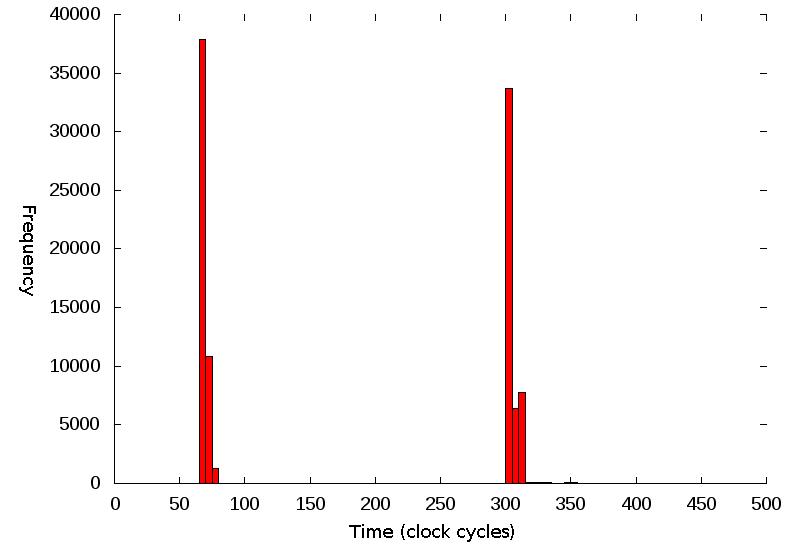
\includegraphics[width=10cm,keepaspectratio]{benchmark.png}
\end{frame}

\begin{frame}[fragile]
    \frametitle{\textsc{Flush+Reload}}
    \framesubtitle{Simple Example}

    \begin{verbatim}
    int main() {
        while (1) {
           foo();
           bar();
        }
    }
    \end{verbatim}

    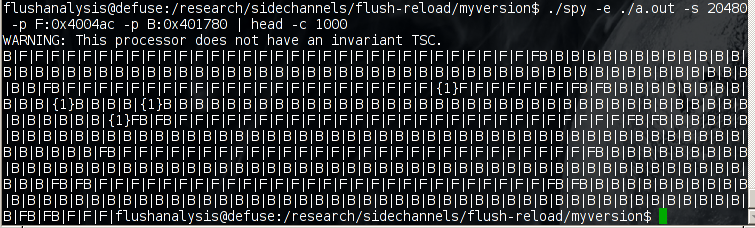
\includegraphics[width=10cm,keepaspectratio]{simpledemo.png}
\end{frame}

\begin{frame}
    \frametitle{\textsc{Flush+Reload}}
    \framesubtitle{Breaking Crypto}

    What can it do?

    \begin{itemize}
        \item \textbf{2011}: Breaks the AES in OpenSSL \footnote{Bangerter et al.}
        \item \textbf{2013}: GnuPG RSA broken (after one decryption!). \footnote{Yuval Yarom and Katrina Falkner}
        \item \textbf{2014}: OpenSSL ECSDA nonce (after one signature!) \footnote{Yuval Yarom and Naomi Benger}
        \item \textbf{2014}: OpenSSL ECDSA private key (after 200 signatures). \footnote{Naomi Benger et al.}
    \end{itemize}

    Really powerful attack!
\end{frame}

\begin{frame}
    \frametitle{\textsc{Flush+Reload}}
    \framesubtitle{More than Crypto?}

    In theory, \textbf{code branch = information leak}

    \begin{itemize}
        \item Which button did the user click?
        \item Vim / Emacs commands?
        \item Email: New mail events. Reply events. (Metadata)
        \item Scripting languages (steal source code?)
    \end{itemize}

    How bad is it? We found two attacks.
\end{frame}

% =============================================================================
% TrueCrypt Attack
% =============================================================================

\begin{frame}
    \frametitle{TrueCrypt Attack}
    \framesubtitle{Goal}

    \begin{center}
    {\Large Attack \#1: TrueCrypt}
    \end{center}
    \begin{columns}
        \begin{column}{0.3\textwidth}
            
\includegraphics[width=4cm,keepaspectratio]{tclogo.png}
        \end{column}
        \begin{column}{0.7\textwidth}
        \begin{itemize}
            \item Full-disk encryption software.
            \item Hidden volumes (coercion defense).
            \item Goal: \textbf{Find out if the volume is hidden.}
        \end{itemize}
        \end{column}
    \end{columns}

    % TODO: put truecrypt screenshot/logo here, maybe hidden volume UI page?
\end{frame}

\begin{frame}
    \frametitle{TrueCrypt Attack}
    \framesubtitle{Implementation 1}

    \begin{itemize}
        \item C++
        \item \texttt{VolumeLayout} classes:
            \begin{itemize}
                \item VolumeLayoutV2\textbf{Normal}
                \item VolumeLayoutV2\textbf{Hidden}
            \end{itemize}
        \item \texttt{GetDataSize()} called on the layout class that works.
        \item Good place for \textsc{Flush+Reload} probes!
    \end{itemize}

\end{frame}

\begin{frame}
    \frametitle{TrueCrypt Attack}
    \framesubtitle{Implementation 2}

    Probes:

    \begin{enumerate}
        \item \texttt{\_start}
        \item \texttt{VolumeLayoutV2Normal::GetDataSize()}
    \end{enumerate}

    Attack:

    \begin{itemize}
        \item Spy on victim mounting the volume.
        \item If probe sequence \textbf{ends} in \texttt{VolumeLayoutV2Normal} hit, output ``normal.''
        \item Otherwise, assume ``hidden.''
    \end{itemize}

\end{frame}

\begin{frame}[fragile]
    \frametitle{TrueCrypt Attack}
    \framesubtitle{It Works (Sort of)}

\begin{verbatim}
    Volume is: normal
    Flush+Reload: S|S|S|S| S|S|R|S|S|S| R|
    Attacker says: normal (right!)

    Volume is: hidden
    Flush+Reload: S|S|S|S|S| S| S|S|S|R|S|S|S|S|S|
    Attacker says: hidden (right!)
\end{verbatim}

    \begin{itemize}
        \item My Laptop: Gets it right over 80\% of the time.
        \item Web Server: Doesn't work!
            \begin{itemize}
                \item Instruction prefetching.
                \item Code is too close together.
            \end{itemize}
    \end{itemize}

\end{frame}

% =============================================================================
% Links Attack
% =============================================================================

\begin{frame}
    \frametitle{Links Attack}
    \framesubtitle{Goal}

    \begin{center}
    {\Large Attack \#2: Links}
    \end{center}
    \begin{columns}
        \begin{column}{0.3\textwidth}
            
\includegraphics[width=3.5cm,keepaspectratio]{linkslogo.png}
        \end{column}
        \begin{column}{0.7\textwidth}
        \begin{itemize}
            \item Command line web browser.
            \item \textbf{Which web page did you just visit?}
            \item Distinguish between the top 100 Wikipedia pages.
        \end{itemize}
        \end{column}
    \end{columns}
\end{frame}

\begin{frame}
    \frametitle{Links Attack}
    \framesubtitle{Implementation 1}

    Probe the HTML parsing code:

    \begin{itemize}
        \item \texttt{parse\_html()}
        \item \texttt{html\_stack\_dup()}
        \item \texttt{html\_h()}
        \item \texttt{html\_span()}
    \end{itemize}

    Trial and error to find the best ones (with Wikipedia in mind).

\end{frame}

\begin{frame}[fragile]
    \frametitle{Links Attack}
    \framesubtitle{Implementation 2}

    Vist the Facebook Wikipedia page, we see...

\begingroup
\fontsize{7pt}{7pt}\selectfont
\begin{verbatim}
HDRDSSSSDSDSDHDHDHDHDRDHDSSDSDSDSDHDHDHDRDRDRDHSRDRDRDRDRDSSDHDRDRDSDSDRDRDRDHDH
DRDHDRDRDRDSDSDSDHSDSRDSDRSSDHSSDSSDSDRDSDSDSDSDSDRDRDHSDSSSDSSRDSDRSSSDHDSDSDRS
DSDSDRDSDRDRDSSDSDSDSDRDSDSDSDSDSDSRDRDSDSDSRDRDRDRDRDSDSRDSDRDRDRDHSDRDRDRDRDRD
RDSDSDRDSDSDRDRDRDRDHSDRDRDSDSDSSDSSDRDRDSSDSSDSDSDRSDRDSSDSDSDSDSDRDSDRDSDSDSDS
RSDRDSHSDSDSDSRDRDSDSSDRDRDSHSDRDSDSRDHSDRDRDRDRSSDSDSDSDRDRDSDSDSDSDSRSRDHSSDSD
SDSDRDSDRDSDSDSSDRDSDRDSDSDSDSDSRDRDSDSDSRDSHSDRDSDSDSDSDRDSDSDSSDSDSDSSDSDSDRDS
RDRDRDRDHDSDRDRDRDRDHDRDRDRDRDRDRDRDRDRDRDRDRDRDRDRDRDRDRDRDRDRDRDRDSHSDRDSDRDHD
RDRHDHSDRDRDSDSSSDSDSDSDRDSDSDSDSDRDSDSDSDSDRDSDSDSDSDRDSDSDSDRSDSDSDRDHDHDSDSDS
DSDSDRDSHDSDSDSDSDSDRDSDSSDRDSDRDRHDSDSDRDSDRDHDSDSDSDSDHSDSSSDSDSSDHDSSSDSDHDHS
DSSDSDSDSSDSDSDSDSDSSSSDSDSSDSDSDSDSDSDSDSDSDSSDSDSDSDSDSSDSDSDSDSDSDSSDSDSDSDSD
SDSDSSDSDSDSDSDSDSDSDSDSDSDSSDSSSDSSDSDSSDSDSDSDSDSDSDSDSDSDSDSDSSDSDSSDSDSDSDSD
SSDSDSSDSSDSDSSDSSDSDSDSDSSDSDSDSDSSDSDSDSDSSDSDSDSDSSDSDSDSDSSDSDSDSSDSDSDSDSDS
SDSSDSDSDSDSSDSDSDSDSDSDSSDSDSSSDSDSDSDSDSDSDSDSDSHSSDSSSDSSDSDSSSDSDSDSDSDSDSDS
DSSDSDSSDSSDSDHDSSDSDHDHDSSDSSDSDSDSSDSDSDSDSDSDSDSDSDRDSSDSDSDSDSDSDSDSDSDSDHSD
SDSDSDSDHSDSDSDSHSDSDSDHSSDSDSDSDSSDSDSDSDSDSDSDHDHDSDSDSDSDSDSDSDSDSDSDSDSDSDSD
SHDHDSDSDSDSDSDHDSDSDSDSDSDSDSDSDSDSDSDSDSDSDSDSDSDSSDSDSSDHDSDSDHSDRDHDSDSDSSDS
DSDSDSDSDSSHSDSSDSDSDSDSDSDSDSDSDSDSDSSDSDSDSDSDSDSDSSDSDSDSDSDSDSDSDSDSDSDHDSDS
DSDSDSDSDHDSSDSDSDSDSDSDSDSDSDSDSDSSDSDSDSDSDSDSDHDSDSDSDSDSDSDHDSDSDSDSDSDSDSDS
SDHSDHDSSDSDSDSDSDSDSDSDSDSDSDSDSDHDSDSDSDSDSSDSDSSDSDSDSDSSDSDSHDSDSDSDSDSDSSDS
DSSDSDSSDSDSDSDSDSDSDSDSDSDSDSDSDSDSDSDSDSDSDSDSDSDSDSSDSDSDSSDSSDSDSDSDSDSDHSDS
DHSHDSSSDSDSDSDRDSDSSDSDSDSDSDSDSDSSDSDSDSDSDHDSSHDSDRDSDRDSSRDRDHDSDSRDRDRDSSDR
DSDSDSRDRDRDSDSRDRDSDSDRDRDSDSDSRDRDSDSRDRDRDRDRDSDSSDRDRDSDSRDRDSDSRDRDRDSDSDSD...
\end{verbatim}
\endgroup
Challenge: \textbf{Identify the page from this string.}

\end{frame}

\begin{frame}
    \frametitle{Links Attack}
    \framesubtitle{Implementation 3}

    Phases of attack:

    \begin{enumerate}
        \item \textbf{Training:} Save 10 samples of each page.
        \item \textbf{Spy on the victim:} Record the victim visiting a page once.
        \item \textbf{Recovery:} Find the ``closest'' sample.
    \end{enumerate}

    ``Closeness'' is measured by Levenshtein distance.
\end{frame}

\begin{frame}
    \frametitle{Links Attack}
    \framesubtitle{Levenshtein Distances}

    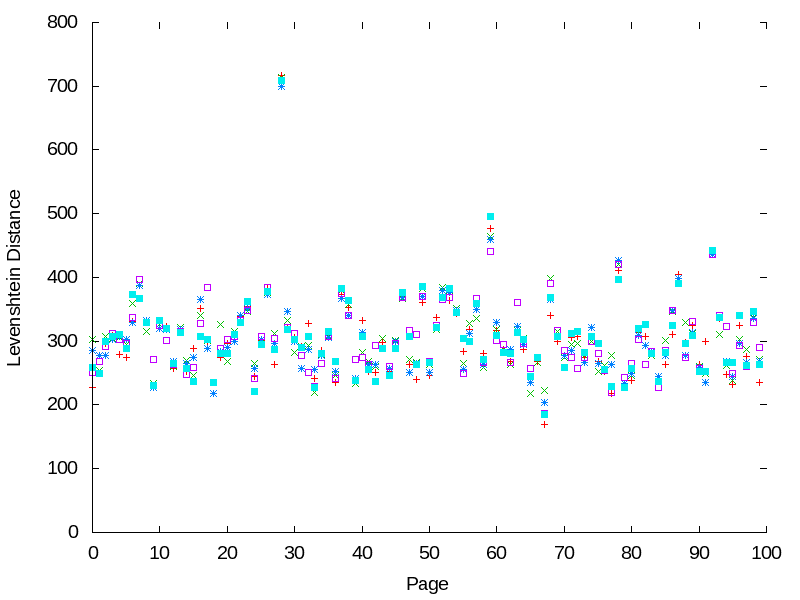
\includegraphics[width=\textwidth,keepaspectratio]{distanceplot.png}

\end{frame}

\begin{frame}
    \frametitle{Links Attack}
    \framesubtitle{It Works}

            \begin{itemize}
                \item Works well on both systems we tried.
                \item \textbf{10 samples: 90\%}
                \item 5 samples: 75\%.
            \end{itemize}
    %\begin{columns}
    %    \begin{column}{0.6\textwidth}
    %        %% GNUPLOT: LaTeX picture
\setlength{\unitlength}{0.240900pt}
\ifx\plotpoint\undefined\newsavebox{\plotpoint}\fi
\sbox{\plotpoint}{\rule[-0.200pt]{0.400pt}{0.400pt}}%
\begin{picture}(750,750)(0,0)
\sbox{\plotpoint}{\rule[-0.200pt]{0.400pt}{0.400pt}}%
\put(151.0,131.0){\rule[-0.200pt]{4.818pt}{0.400pt}}
\put(131,131){\makebox(0,0)[r]{ 0}}
\put(669.0,131.0){\rule[-0.200pt]{4.818pt}{0.400pt}}
\put(151.0,247.0){\rule[-0.200pt]{4.818pt}{0.400pt}}
\put(131,247){\makebox(0,0)[r]{ 10}}
\put(669.0,247.0){\rule[-0.200pt]{4.818pt}{0.400pt}}
\put(151.0,362.0){\rule[-0.200pt]{4.818pt}{0.400pt}}
\put(131,362){\makebox(0,0)[r]{ 20}}
\put(669.0,362.0){\rule[-0.200pt]{4.818pt}{0.400pt}}
\put(151.0,478.0){\rule[-0.200pt]{4.818pt}{0.400pt}}
\put(131,478){\makebox(0,0)[r]{ 30}}
\put(669.0,478.0){\rule[-0.200pt]{4.818pt}{0.400pt}}
\put(151.0,593.0){\rule[-0.200pt]{4.818pt}{0.400pt}}
\put(131,593){\makebox(0,0)[r]{ 40}}
\put(669.0,593.0){\rule[-0.200pt]{4.818pt}{0.400pt}}
\put(151.0,709.0){\rule[-0.200pt]{4.818pt}{0.400pt}}
\put(131,709){\makebox(0,0)[r]{ 50}}
\put(669.0,709.0){\rule[-0.200pt]{4.818pt}{0.400pt}}
\put(175,131){\usebox{\plotpoint}}
\put(175,709){\usebox{\plotpoint}}
\put(175,90){\makebox(0,0){10}}
\put(224,131){\usebox{\plotpoint}}
\put(224,709){\usebox{\plotpoint}}
\put(224,90){\makebox(0,0){9}}
\put(273,131){\usebox{\plotpoint}}
\put(273,709){\usebox{\plotpoint}}
\put(273,90){\makebox(0,0){8}}
\put(322,131){\usebox{\plotpoint}}
\put(322,709){\usebox{\plotpoint}}
\put(322,90){\makebox(0,0){7}}
\put(371,131){\usebox{\plotpoint}}
\put(371,709){\usebox{\plotpoint}}
\put(371,90){\makebox(0,0){6}}
\put(420,131){\usebox{\plotpoint}}
\put(420,709){\usebox{\plotpoint}}
\put(420,90){\makebox(0,0){5}}
\put(469,131){\usebox{\plotpoint}}
\put(469,709){\usebox{\plotpoint}}
\put(469,90){\makebox(0,0){4}}
\put(518,131){\usebox{\plotpoint}}
\put(518,709){\usebox{\plotpoint}}
\put(518,90){\makebox(0,0){3}}
\put(567,131){\usebox{\plotpoint}}
\put(567,709){\usebox{\plotpoint}}
\put(567,90){\makebox(0,0){2}}
\put(616,131){\usebox{\plotpoint}}
\put(616,709){\usebox{\plotpoint}}
\put(616,90){\makebox(0,0){1}}
\put(665,131){\usebox{\plotpoint}}
\put(665,709){\usebox{\plotpoint}}
\put(665,90){\makebox(0,0){0}}
\put(151.0,131.0){\rule[-0.200pt]{0.400pt}{139.240pt}}
\put(151.0,131.0){\rule[-0.200pt]{129.604pt}{0.400pt}}
\put(689.0,131.0){\rule[-0.200pt]{0.400pt}{139.240pt}}
\put(151.0,709.0){\rule[-0.200pt]{129.604pt}{0.400pt}}
\put(30,420){\makebox(0,0){\rotatebox{90}{Number of pages}}}
\put(420,29){\makebox(0,0){Times correctly identified of 10}}
\put(151.0,131.0){\rule[-0.200pt]{0.400pt}{119.727pt}}
\put(151.0,628.0){\rule[-0.200pt]{11.804pt}{0.400pt}}
\put(200.0,131.0){\rule[-0.200pt]{0.400pt}{119.727pt}}
\put(151.0,131.0){\rule[-0.200pt]{11.804pt}{0.400pt}}
\put(200.0,131.0){\rule[-0.200pt]{0.400pt}{91.783pt}}
\put(200.0,512.0){\rule[-0.200pt]{11.804pt}{0.400pt}}
\put(249.0,131.0){\rule[-0.200pt]{0.400pt}{91.783pt}}
\put(200.0,131.0){\rule[-0.200pt]{11.804pt}{0.400pt}}
\put(249.0,131.0){\rule[-0.200pt]{0.400pt}{22.163pt}}
\put(249.0,223.0){\rule[-0.200pt]{11.804pt}{0.400pt}}
\put(298.0,131.0){\rule[-0.200pt]{0.400pt}{22.163pt}}
\put(249.0,131.0){\rule[-0.200pt]{11.804pt}{0.400pt}}
\put(298.0,131.0){\rule[-0.200pt]{0.400pt}{19.513pt}}
\put(298.0,212.0){\rule[-0.200pt]{11.804pt}{0.400pt}}
\put(347.0,131.0){\rule[-0.200pt]{0.400pt}{19.513pt}}
\put(298.0,131.0){\rule[-0.200pt]{11.804pt}{0.400pt}}
\put(347.0,131.0){\rule[-0.200pt]{0.400pt}{11.081pt}}
\put(347.0,177.0){\rule[-0.200pt]{11.804pt}{0.400pt}}
\put(396.0,131.0){\rule[-0.200pt]{0.400pt}{11.081pt}}
\put(347.0,131.0){\rule[-0.200pt]{11.804pt}{0.400pt}}
\put(396.0,131.0){\rule[-0.200pt]{0.400pt}{5.541pt}}
\put(396.0,154.0){\rule[-0.200pt]{11.563pt}{0.400pt}}
\put(444.0,131.0){\rule[-0.200pt]{0.400pt}{5.541pt}}
\put(396.0,131.0){\rule[-0.200pt]{11.563pt}{0.400pt}}
\put(493.0,131.0){\rule[-0.200pt]{0.400pt}{2.891pt}}
\put(493.0,143.0){\rule[-0.200pt]{11.804pt}{0.400pt}}
\put(542.0,131.0){\rule[-0.200pt]{0.400pt}{2.891pt}}
\put(493.0,131.0){\rule[-0.200pt]{11.804pt}{0.400pt}}
\put(542.0,131.0){\rule[-0.200pt]{0.400pt}{2.891pt}}
\put(542.0,143.0){\rule[-0.200pt]{11.804pt}{0.400pt}}
\put(591.0,131.0){\rule[-0.200pt]{0.400pt}{2.891pt}}
\put(542.0,131.0){\rule[-0.200pt]{11.804pt}{0.400pt}}
\put(640.0,131.0){\rule[-0.200pt]{0.400pt}{2.891pt}}
\put(640.0,143.0){\rule[-0.200pt]{11.804pt}{0.400pt}}
\put(689.0,131.0){\rule[-0.200pt]{0.400pt}{2.891pt}}
\put(640.0,131.0){\rule[-0.200pt]{11.804pt}{0.400pt}}
\put(151.0,131.0){\rule[-0.200pt]{0.400pt}{139.240pt}}
\put(151.0,131.0){\rule[-0.200pt]{129.604pt}{0.400pt}}
\put(689.0,131.0){\rule[-0.200pt]{0.400pt}{139.240pt}}
\put(151.0,709.0){\rule[-0.200pt]{129.604pt}{0.400pt}}
\end{picture}

    %    \end{column}
    %    \begin{column}{0.4\textwidth}
    %    \end{column}
    %\end{columns}
\end{frame}

\begin{frame}
    \frametitle{Links Attack}
    \framesubtitle{Demo}

    \begin{center}
    {\Large Demo!}
    \end{center}
\end{frame}


% =============================================================================
% Conclusion
% =============================================================================

\begin{frame}
    \frametitle{Conclusion}

    \begin{itemize}
        \item These are \textbf{boring attacks}.
        \begin{itemize}
            \item TrueCrypt: 1 bit.
            \item Links: $\log_2(100) = 6.6$ bits.
        \end{itemize}
        \item But shows \textsc{Flush+Reload} is bad for privacy.
        \item Deserves more research!
        \item Can we automate it?
            \begin{itemize}
                \item Try all of those ideas...
                \item Defense: Can we distinguish between private keys?
            \end{itemize}
    \end{itemize}
\end{frame}

\begin{frame}
    Thanks for listening! Questions?
\end{frame}

\end{document}
